
\chapter{Introduction}
\label{chap:introduction}

\section{Problem Statement}
\label{sec:introduction:probstatement}


Rate control is crucial for the performance of WiFi networks.
However, the absence of an effective analytical tool restricts the visualization and comprehension of various factors exploiting rate selection and data transmission performance. Current research~\cite{8548800} is focusing more on offering optimization solutions based on simulation rather than real-world scenarios. Therefore, there is a limited investigation into the capabilities and adaptability of the Minstrel-HT algorithm in real-world scenarios with network congestion, and high levels of network activity. Without an effective analytical tool, it's difficult to visualize and understand the factors that impact rate selection and data transmission performance, it also restricts the identification of optimization opportunities. 
It is necessary to have a tool that can create analytical plots that cover different aspects, including the number of transmitted data frames, the number of successful and failed transmissions by frame count and the probability of them. This will help to gain a deeper comprehension of the process of transmitting data, In addition to that, the details of network performance.




\section{Contributions}
\label{sec:introduction:contrib}

The current thesis Introduces Minstrel-HT rate selection algorithm, providing a clear understanding of how data rates are determined based on channel conditions and supported WiFi standards. This contribution enhances our knowledge of MCS schemes, and rate control algorithms in wireless networks and general Minstrel-HT rate selection methods. Moreover focuses on the data collection setup and monitoring information format which been used in the analysis. By analyzing trace files extracted from the Linux kernel, it provides information about rates and network performance. The precise description of each trace line improves our understanding of the data transmission process~\ref{chap:Measurement Tools}.
For this purpose, the thesis presents a Python-based tool~\ref{chap:Analysis and Optimization}that enables the generation of analytical plots for quantitative analysis. The tool provides deeper insights into available rates such as; per Station, Number of transmitted data frames, Number of successful and failed transmissions and probability of them and more. Also, performance evaluation of real-world scenarios was executed to evaluate the capabilities of the tool.

\section{WiFi data transmission rate - MCS Index}
\label{sec:intro:WiFi-MCS}

The Modulation and Coding Scheme (MCS)~\cite{MCS-Index} is a list of available coding and modulation schemes used by WiFi devices to transmit data packets. The MCS index defines data rates in accordance with the 802.11n (HT), 802.11ac (VHT), and 802.11ax (HE) standards and capabilities. Each standard introduces new data rates based on varying WiFi variables. This formula can be utilized to calculate the data rate used for both 802.11n and 802.11ac wireless communication standards.
\vspace{2cm}
\begin{align*}
\textbf{\large Data Rate} &= \frac{\textbf{N}_{\text{SD}} \times \textbf{N}_{\text{BPSCS}} \times \textbf{R} \times \textbf{N}_{\text{SS}}}{\textbf{T}_{\text{DFT}} + \textbf{T}_{\text{GI}}}
\end{align*}
\begin{itemize}
    \item $\textbf{N}_{\text{SD}}$: Number of Data Sub-carriers
    \item $\textbf{N}_{\text{BPSCS}}$: Number of Code Bits per Sub-carrier Per Stream
    \item $\textbf{R}$ : Coding
    \item $\textbf{N}_{\text{SS}}$: Number of Spatial Streams
    \item $\textbf{T}_{\text{DFT}}$: OFDM Symbol Duration
    \item $\textbf{T}_{\text{GI}}$: Guard Interval Duration
\end{itemize}
\vspace{2cm}
\clearpage
\begin{figure}[hbt!]  
    \centering
    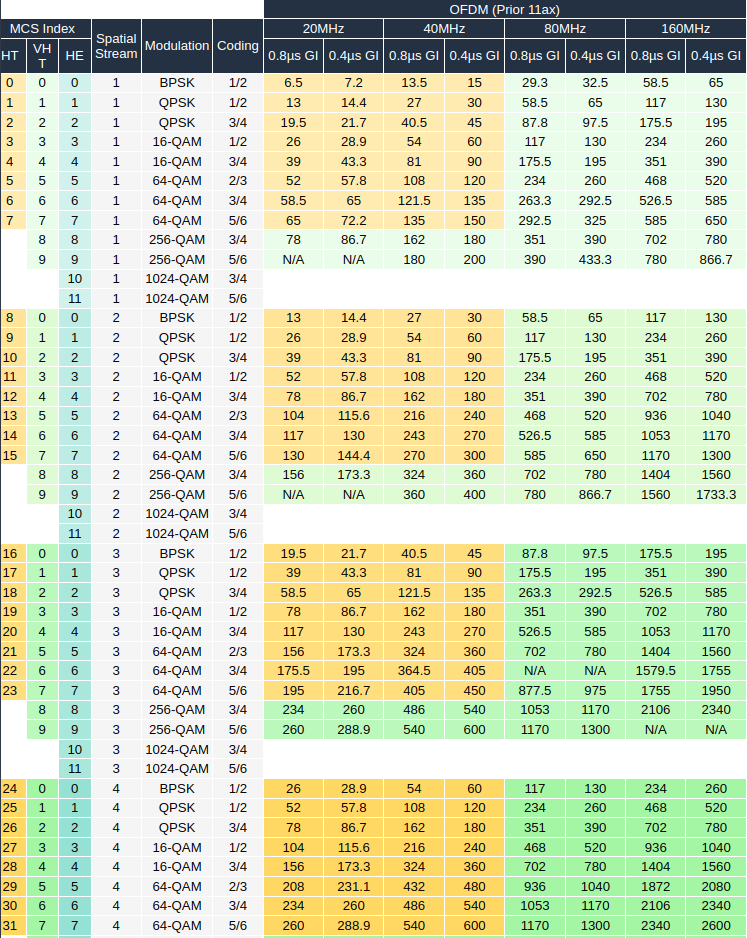
\includegraphics[width=\textwidth]{figures/MCS-Index.png}
    \caption{MCS Index}
    \label{fig:plot_MCS_Index}
\end{figure}
\FloatBarrier
\vspace{1cm}
MCS Index refers to the values used to differentiate the various modulation and coding schemes supported by the 802.11n (HT), 802.11ac (VHT), and 802.11ax (HE) standards. In the table, these values are represented by different colors which indicate the different levels of modulation and coding schemes supported by each standard. This method offers an easy way to identify the most appropriate modulation and coding scheme to use for a given wireless communication link based on the current channel conditions and the supported Wi-Fi standard.

Modulation schemes have different levels of complexity and can achieve different data rates and performance under various channel conditions.
For example, for 802.11ac (VHT), the modulation column indicates the following modulation schemes: 
\begin{itemize}
    \item BPSK (Binary Phase Shift Keying)
    \item QPSK (Quadrature Phase Shift Keying)
    \item 16-QAM (Quadrature Amplitude Modulation)
    \item 64-QAM (Quadrature Amplitude Modulation)
    \item 256-QAM (Quadrature Amplitude Modulation). 
\end{itemize}    
Each modulation scheme corresponds to a different number of bits per symbol, which determines the maximum data rate that can be achieved for a given signal bandwidth and signal-to-noise ratio (SNR)~\cite{proakis2008digital}.
Coding refers to the way that digital data is encoded before transmission over the wireless channel. 
Coding is used to improve the reliability of wireless communication by adding redundancy to the transmitted data, which allows for error detection and correction. Coding rate of 3/4~means that for every 4~bits of information that are transmitted, an additional 3 bits of redundancy are added. This results in a total of 7~bits being transmitted for every 4~bits of original data, which corresponds to a coding rate of 3/4~\cite{rappaport-2002}.

The different Wi-Fi standards support different channel bandwidths. Specifically, 802.11n (HT) supports channel bandwidths of 20~MHz and 40~MHz, while 802.11ac (VHT) supports channel bandwidths of 20~MHz, 40~MHz, 80~MHz, and 160~MHz. The latest Wi-Fi standard, 802.11ax (HE), supports more channel bandwidth options, including 20~MHz, 40~MHz, 80~MHz, 80+80~MHz, and 160~MHz. The choice of channel bandwidth for a given wireless network depends on various factors, such as the desired data rate, the available spectrum, and the level of interference.

Guard Interval (GI) is a parameter used to separate individual symbols transmitted in a wireless signal to prevent inter-symbol interference. In 802.11n~(HT), GI values are 400~ns for 20~MHz channels and 800~ns for 40~MHz channels. In 802.11ac~(VHT), GI values are 400~ns for 20~MHz, 40~MHz, and 80~MHz channels, and 1600~ns for 160~MHz channels. For 802.11ax (HE), GI values are 400~ns for all channels, and 3200~ns for 80+80~MHz channels. The choice of GI value affects the duration of the guard interval and can impact the overall throughput of the wireless network. Therefore, it is an important parameter to consider when designing and optimizing a wireless network~\cite{rappaport-2002}.
The number of spatial streams indicates the number of independent data streams that can be transmitted simultaneously in a wireless communication system. For 802.11n~(HT) supports up to four, 802.11ac~(VHT) supports up to eight, and 802.11ax~(HE) supports up to twelve spatial streams.The number of spatial streams a Wi-Fi standard supports represents the theoretical maximum number of independent data streams that can be transmitted at once. However, the actual number of spatial streams that can be used in practice depends on factors like the radio environment, antenna configuration, and processing capabilities of the transmitter and receiver.


\section{WiFi Rate Control - Minstrel HT}
\label{sec:intro:wifiratecontrol:MinstrelHT}

Minstrel-HT~\cite{MinstrelHT(2010)} is an advanced wireless rate control algorithm that expands upon the original Kernel Minstrel algorithm~\cite{MinstrelKernel} to support the IEEE 802.11n and 802.11ac Wi-Fi standards. The algorithm uses a heuristic statistical model to find the best transmission rate for a wireless channel. It calculates the success probability of each possible transmission rate for each antenna stream, channel bandwidth, guard interval, and modulation coding scheme combination. This method helps Minstrel-HT choose the better data rates, which increases performance. The algorithm operates a feedback mechanism that enables it to adapt to changing network conditions over time. The algorithm continuously monitors the rate statistics~\ref{intro:Rate Statistic Calculation} of each transmission rate and updates its estimation models accordingly. This is achieved through a reinforcement learning algorithm that adjusts the success probability estimates based on the observed outcomes of each transmission~\cite{liu2014minstrelht}.


\subsection{Group Creation and Rate Definition in Minstrel-HT}
\label{sec:intro:wifiratecontrol:Group creation}

The definitions provided in Section~\ref{sec:intro:WiFi-MCS}, the MCS Index define a metric that considers multiple parameters related to the Wi-Fi connection established between a client device and a wireless access point. Throughout this thesis and in the upcoming chapters, the Minstrel-HT rate table is used for a more accurate analysis. Our experiments will specifically be using the ath9k chipset that is provided with high throughput (HT) rates only, as shown in~\ref{tab:3b}. The table provides information related to the Bandwidth, availability of a long/short guard interval, and the number of spatial streams. Within each group rate, the same specifications are shared, for example, for rates within group C, the bandwidth, long guard interval, and spatial streams are the same, what makes $C_{0}$, $C_{1}$ and $C_{7}$ different, is the modulation and coding schemes (MCS).

The Minstrel-HT algorithm calculates the transmission time for each Modulation and Coding Scheme (MCS) based on channel conditions. When selecting an MCS for a particular transmission, it is crucial to consider the duration of the transmission. The value in~\ref{tab:3b} represents the transmission time for the raw data part of an average-sized packet~\ref{item:AVG_PKT_SIZE}, for a given MCS, guard interval, and channel bandwidth. The algorithm takes into account the number of streams, the guard interval type (short or long), and the number of bits per symbol as input variables. The output of this algorithm is the transmission time in unit nanoseconds. This transmission time which is referred to it as is displayed in the table as a hexadecimal value and in the scope of this thesis it referred to as the airtime value. The MCS with the lowest airtime value is typically chosen to achieve the highest data rate successful transmissions while maintaining the required level of reliability. However, the MCS with the highest airtime value is chosen for transmissions with poor channel conditions to improve the reliability of the transmission.


\begin{landscape}
\begin{table}[ht]
    \centering
    \begin{tabular}{||c c c c c c c c c c c c c c c c c c c||} 
         \hline
         Group& Type & BW & SGI & NSS & BPSK1/2 & QPSK1/2 & QPSK3/4 & 16-QAM1/2 & 16-QAM3/4 & 64-QAM2/3 & 64-QAM3/4 & 64-QAM5/6  \\ [0.5ex] 
         \hline
         0 & ht & 1 & 0 & 0 & 168980 & b44c0 & 783c0 & 5a260 & 3c1e0 & 2d1a0 & 28180 & 24120  \\ 
         \hline
         1 & ht & 2 & 0 & 0 & b44c0 & 5a260 & 3c1e0 & 2d1a0 & 1e170 & 16950 & 14140 & 12110 \\
         \hline
         2 & ht & 3 & 0 & 0 & 783d0 & 3c1e8 & 28198 & 1e170 & 14148 & f130 & d5d8 & c060 \\
         \hline
         3 & ht & 4 & 0 & 0 & 5a260 & 2d1a8 & 1e170 & 16950 & f130 & b4a8 & a120 & 9088 \\
         \hline
         4 & ht & 1 & 0 & 1 & 1448c0 & a2460 & 6c3a0 & 51240 & 361e0 & 289a0 & 241a0 & 207a0 \\ 
         \hline
         5  & ht & 2 & 0 & 1 & a2470 & 51250 & 361e0 & 289b0 & 1b170 & 14560 & 12150 & 10450 \\
         \hline
         6 & ht & 3 & 0 & 1 & 6c3a0 & 361e8 & 241a0 & 1b178 & 12158 & d948 & c0a8 & ad50\\
         \hline
         7 & ht & 4 & 0 & 1 & 51250 & 289b0 & 1b178 & 14560 & d948 & a2c8 & 9130 & 8240\\
         \hline
         8 & ht & 1 & 1 & 0 & ada50 & 56da0 & 39ec0 & 2b750 & 1cfd0 & 15ba0 & 13590 & 11650\\
         \hline
         9 & ht & 2 & 1 & 0 & 56da0 & 2b750 & 1cfd8 & 15ba8 & e868 & add0 & 9b40 & 8ba0\\
         \hline
         a & ht & 3 & 1 & 0 & 39ec0 & 1cfdc & 13590 & e86c & 9b44 & 7434 & 6784 & 5cc4\\
        \hline
        b & ht & 4 & 1 & 0 & 2b750 & 15ba8 & e86c & add4 & 7434 & 56e8 & 4e20 & 4650\\
        \hline
        c & ht & 1 & 1 & 1 & 9c4a0 & 4e2e0 & 34240 & 271f0 & 1a1a0 & 13910 & 116c0 & faa0\\
        \hline 
        d & ht & 2 & 1 & 1 & 4e2e0 & 271f8 & 1a1a8 & 13910 & d160 & 9ca0 & 8bf0 & 7de0\\
        \hline
        e & ht & 3 & 1 & 1 & 34244 & 1a1ac & 116cc & d160 & 8bf0 & 68c8 & 5d5c & 53b0\\
        \hline
        f & ht & 4 & 1 & 1 & 271f8 & 13914 & d160 & 9ca4 & 68c8 & 4e68 & 4680 & 3f78\\
        \hline
        10 & cck & 1 & 0 & 0 & 960e00 & 4c9100 & 1dcc00 & 106f00 & 949700 & 4b1a00 & 1c5500 & ef800\\
        \hline
        11 & ofdm & 1 & 0 & 0 & 190640 & 10d880 & cc1a0 & 8aac0 & 6a720 & 493e0 & 399e0 & 33c20\\
    \end{tabular}
    \caption[Minstrel-HT Rate Group]{Minstrel-HT Rates are presented in the table with details including the Group number, Type of modulation techniques, Bandwidth, Short Guard Interval, Number of spatial streams, and Modulation schemes.}\label{tab:3b}
  \end{table}  
\end{landscape}








\subsection{Rate Sampling (Probing)}
\label{sec:intro:minstrelht:probing}
The requirement for rate sampling arises due to the dynamic nature of the wireless channel's quality, which fluctuates over time. To achieve the maximum possible throughput, it is essential to select a suitable transmission rate that maximizes the data transfer rate and minimizes the failure of transferred rate. Minstrel-HT achieves this goal by probing the channel periodically ,the packets contain no data but the purpose is to collect information regarding to channel quality.The period of updating sampling queue is 50~Hz (20~milliseconds),During each channel update sampling queue updates occurs 2~times. 

Minstrel-HT~\cite{MinstrelHT(2010)} employs three different sampling strategies: increment, jump, and slow. To construct the rate table for each strategy, up to five rates are stored in a queue and pushed out in a First-in-First-out~(FIFO) sequence when the algorithm requests a probing rate. The sequence in which these strategies are employed follows:
\begin{lstlisting}
    Increment
    Jump
    Increment
    Jump
    Increment
    Slow
\end{lstlisting}
The sequence goes into a loop if all the rates in the queue have been probed.
\begin{itemize}
    \item Increment: By conducting an incremental search across groups~\ref{sec:intro:wifiratecontrol:Group creation}, chooses a faster rate than maximum throughput. Upon the next iteration of incremental search, the algorithm will resume from the group that immediately follows the one where the faster rate was identified.
    \item Jump: The process of determining rates in a random manner, followed by the selection of rates that surpass the current highest selected rate(faster than maximum throughput). The search for rates in groups is done sequentially, but the selection process involves drawing an index from a global sample table that was randomly constructed. This index is located using the row and column indices associated with the group. The search ends when a rate that is faster than the maximum throughput is found.
    \item Slow: Rates that lie within the spectrum of the fastest and slowest rates are allocated to the slow sample bucket, given that adequate space is available. Here's what happens if the rates are faster than the slowest of (seconds maximum throughput and max success probability)
\end{itemize}



At every statistical update, which occurs at a frequency of 20~Hz (50~ms), the probing queues are replenished with new rates. In instances where data transmission speed and traffic are low, all rates within the queues are utilized. However, when the next statistical update occurs, rates in the queues are deemed unsuitable for sampling, as the channel environment may have changed. As a result, any remaining rates in the queues will be shifted to the front and removed before being replaced with new rates.
When data transmission speed and traffic are low,some rates will remain in the queues,not been sampled. However, in the event that the channel conditions have changed by the time the next statistical update occurs, the rates in the queues may no longer be suitable for probing. This is because the channel environment is constantly changing due to various factors, such as the presence of other wireless devices and the physical location of the transmitter and receiver. As a result, any remaining rates in the queues that are deemed unsuitable for sampling will be shifted to the front and removed before being replaced with new rates that are more reflective of the current channel conditions.



\subsection{Rate Selection in Multi-Rate-Retry(MRR)Chain}

The Multi Rate Retry (MRR) algorithm in Minstrel-HT selects the optimal transmission rate and retry count based on the channel conditions to maximize the successful transmission rate. The MRR algorithm constructs a rate retry chain that specifies which transmission rates to attempt and how many times, based on the estimated success probabilities and the retry limits. It starts by estimating the success probability of each transmission rate for every antenna stream and channel bandwidth combination, using a heuristic statistical model. Once the success probabilities are estimated, the MRR algorithm constructs the rate retry chain that lists the available transmission rates and the corresponding retry limits,the maximum number of retries is determined by the MAX-RETRIES constant,that shows how many times the algorithm should attempt for each rate. The algorithm then selects the first rate in the chain and attempts to transmit the packet at that rate. If the packet is successfully transmitted, the algorithm continues to use that rate for subsequent packets until the channel conditions change. 

In this context for calculating estimated values, constants are being used as follows: the average size of the A-MPDU (Aggregate MAC Protocol Data Unit) is defined as 16, which means the average A-MPDU size used in the Minstrel-HT algorithm is 16~packets. This value is used to calculate the duration of an A-MPDU, which is a collection of packets that are transmitted in a single transmission opportunity. The other constant is  AVG-PKT-SIZE (Average packet size)~\label{item:AVG_PKT_SIZE} which is defined as 1200, which means the average packet size used in the Minstrel-HT algorithm is 1200~bytes. This value is used to estimate the number of packets that can be transmitted in a given duration, taking into account the different transmission rates available.

If the packet is not successfully transmitted, the MRR algorithm moves on to the next rate in the chain and attempts to transmit the packet at that rate, using the retry limit for that rate. If the packet is still not successfully transmitted after all the retries for that rate, the algorithm moves on to the next rate in the chain and repeats the process until either the packet is successfully transmitted or all the rates in the chain have been tried.

\subsection{Rate Statistic Calculation}
\label{intro:Rate Statistic Calculation}
\begin{figure}[htbp]
  \centering
  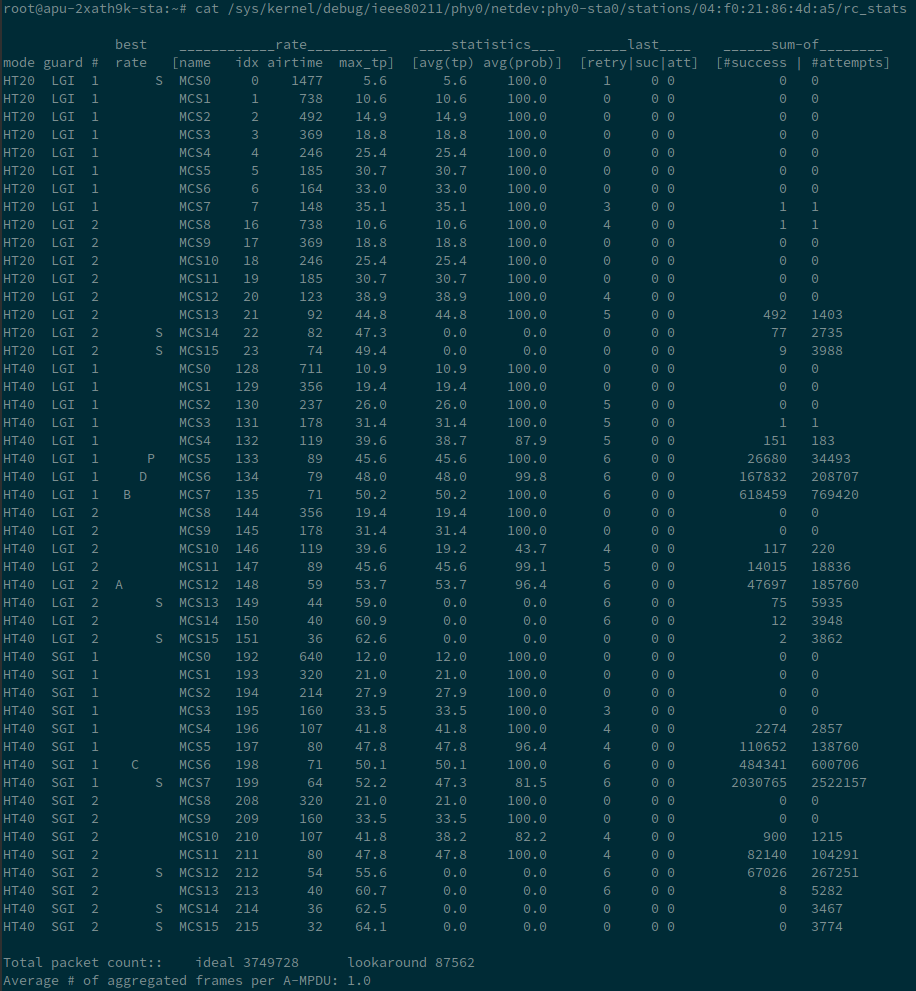
\includegraphics[width=\textwidth]{figures/stats.png}
  \caption[Minstrel-HT rate statistics]{Minstrel-HT rate statistics for ath9k driver APU2E4 AP  }
  \label{fig:rate_statistics}
\end{figure}


In Minstrel-HT, the rate statistical update mechanism is an essential component of the system, responsible for keeping track of the performance of different rates over time and updating their expected throughput values. This mechanism monitors the observed packet transmission rates for each available MCS over a specific period and calculates a weighted moving average. The current version of Minstrel-HT performs statistical updates every 20~Hz (50~ms).

For each associated station, Minstrel-HT tracks the observed performance of utilized rates by maintaining a list of the top four rates with the highest expected throughput and the rate with the highest success probability for each rate group. Counters are also kept for attempted and successful transmissions during the current and previous update periods, as well as the previous two periods' success probabilities for each individual rate. By analyzing this information along with low-pass filtering, Minstrel-HT can make more accurate and reliable decisions about which MCS to use for a given transmission, ultimately leading to improved overall performance and throughput.

In previous Minstrel-HT~\cite{MinstrelHT(2010)} algorithm, to obtain a more accurate calculation, the observed rate performances needed to be averaged. The Estimated Weighted Moving Average (EWMA) method was previously used to achieve this. EWMA is a type of average that assigns different weights to each data point in a set, depending on its relative importance.
In the current Minstrel-HT~\cite{MinstrelHT-patch}, a 2-pole Butterworth low-pass filter is utilized to improve the accuracy of the rate statistical update mechanism. The filter smooths out observed packet transmission rates, filters out high-frequency noise and fluctuations, and provides a gradual and smooth transition between the pass-band and the stop-band. The filter is an important component to achieve accurate rate selection decision by Minstrel-HT.
\newpage
\section{Summary}


This chapter covers the problem statement~\ref{sec:introduction:probstatement} and contribution~\ref{sec:introduction:contrib}. It also includes an introduction to MCS Index and the formula for calculating the data rate, which is described in~\ref{sec:intro:WiFi-MCS}. 
Additionally, section~\ref{sec:intro:wifiratecontrol:MinstrelHT} explains how minstrel rates are inspired and calculated from the MCS index, and the Minstrel algorithm rate sampling for optimization enhancement. It also explores the main strategies (slow, increment, jump) and introduces the Multi Rate Retry chain and statistic update mechanism.